\begin{frame}{HyPer}
The overview of HyPer
\begin{itemize}
\item HyPer targets main-memory database
\item HyPer compiles SQL to LLVM
\item HyPer mixes LLVM and C++ before generating machine code
\end{itemize}
\begin{figure}[htb]

\includegraphics[width=0.4\textwidth]{fig/hyper-logo.png}
\end{figure}
\end{frame}

\begin{frame}{HyPer: An Example}
A simple example
\begin{figure}[htb]
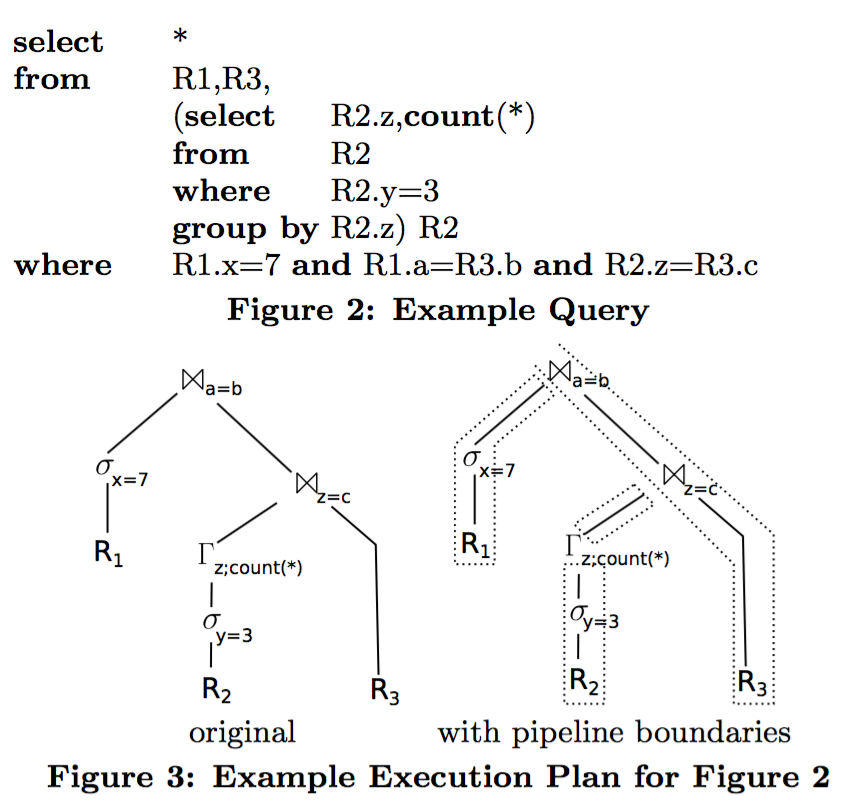
\includegraphics[width=0.5\textwidth]{fig/hyper-fig2.png}
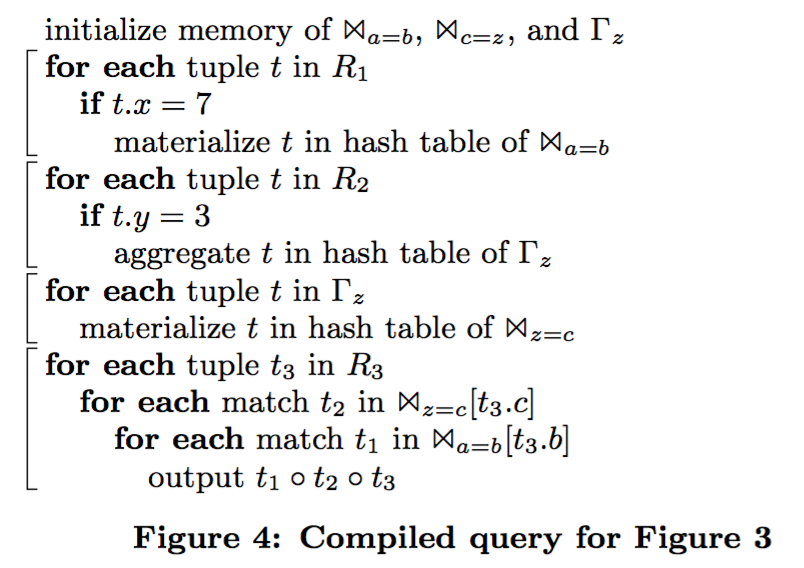
\includegraphics[width=0.5\textwidth]{fig/hyper-fig4.png}
\end{figure}
\end{frame}

\begin{frame}{HyPer: Evaluation}
Show the OLAP part (online analytic processing)
\begin{figure}[htb]
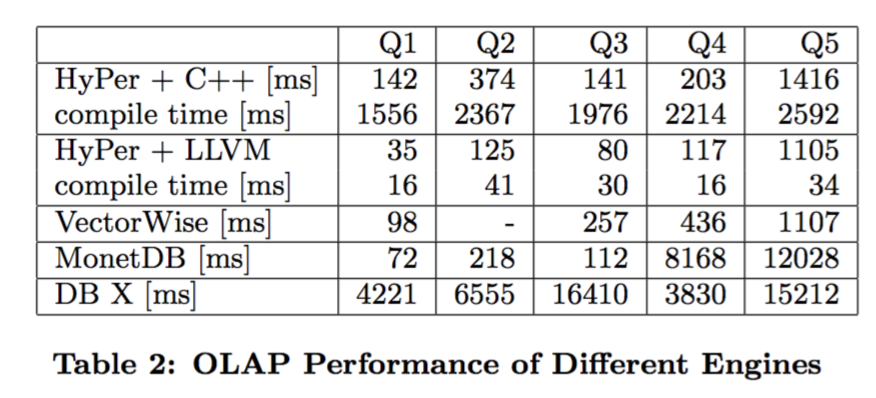
\includegraphics[width=0.6\textwidth]{fig/hyper-table2.png}
\end{figure}
\begin{itemize}
\item TPC-H benchmarks: Q1-5
\item HyPer + LLVM has significantly low compile time
\end{itemize}
\end{frame}

% Start adaptive execution

\begin{frame}{HyPer: Adaptive Execution}
Adaptive execution is necessary, when
\begin{itemize}
\item processing many complex but quick queries, because compiling complex
      queries usually may take hundreds of milliseconds.
\end{itemize}
\pause
Possible applications
\begin{itemize}
\item Streaming/real-time queries
\end{itemize}
\pause
Implementation
\begin{itemize}
\item Kohn et al. implemented a fast bytecode interpreter for LLVM to save the costly compile time
\end{itemize}
\end{frame}

\begin{frame}{Adaptive Execution}
Architecture of compilation-based query engines
\begin{figure}[htb]
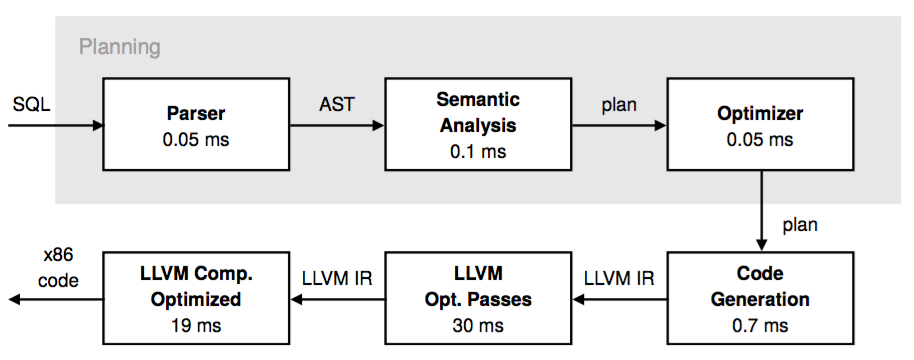
\includegraphics[width=0.6\textwidth]{fig/adaptive-fig1.png}
\end{figure}
\begin{itemize}
\item LLVM optimizations dominate the whole pipeline (very expensive!)
\end{itemize}
\end{frame}

\begin{frame}{Adaptive Execution}
Three modes: 1) LLVM Opt. 2) LLVM Unopt. and 3) Byte Code Compiler
\begin{figure}[htb]
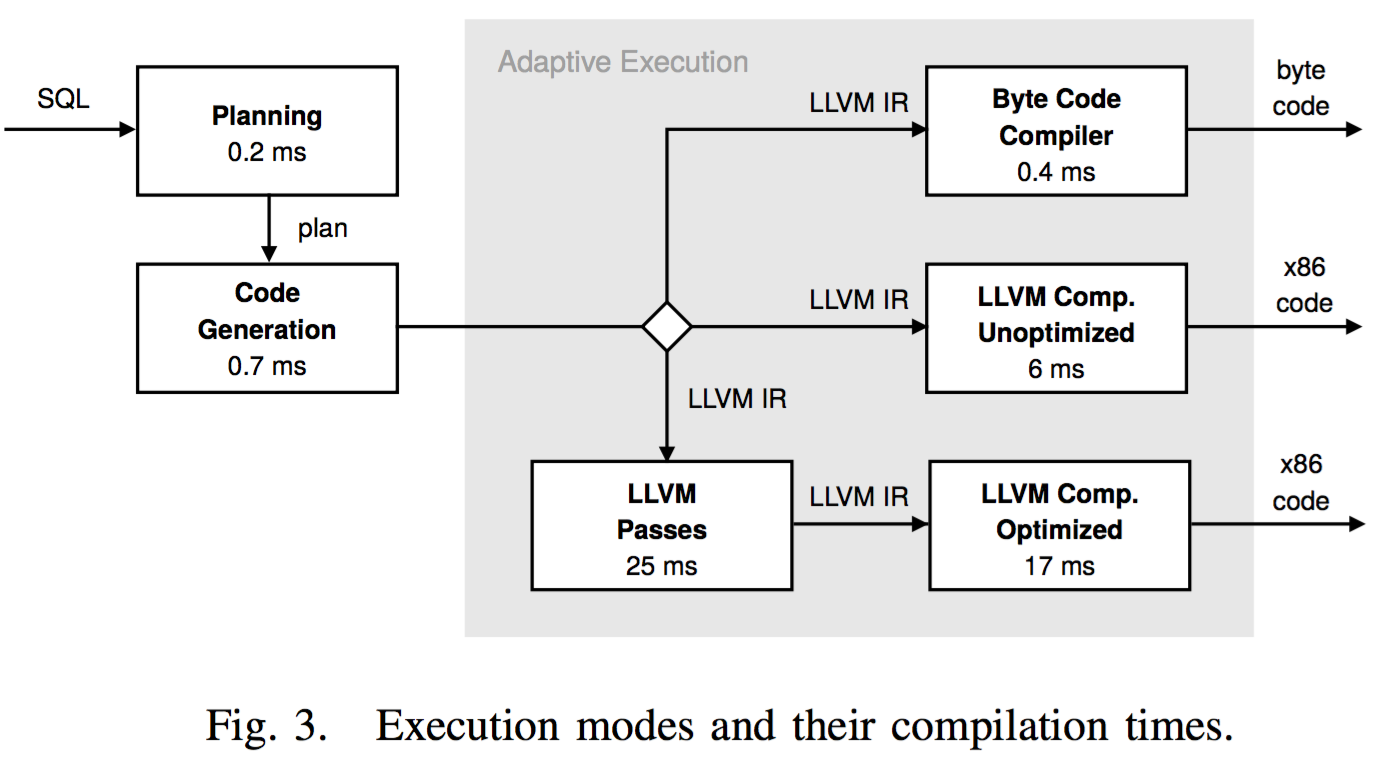
\includegraphics[width=0.8\textwidth]{fig/adaptive-fig3.png}
\end{figure} 
\end{frame}

\begin{frame}{Execution Modes}
The challenge question is how to switch between three modes seamlessly.
\begin{itemize}
\item Split an query into smaller units, called \hgb{morsels}
\item Switch between morsels which are the \hgr{smallest} units
\end{itemize}
\end{frame}

\begin{frame}{Execution Modes}
Switch on-the-fly
\begin{figure}[htb]
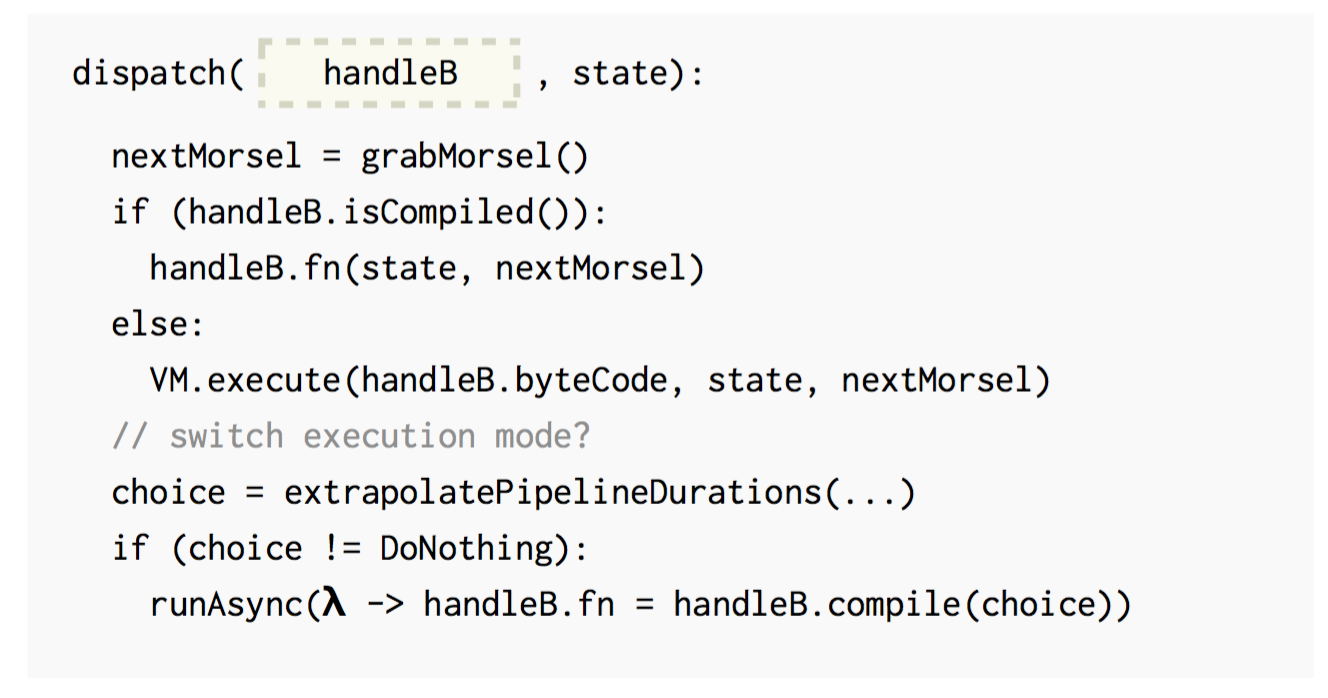
\includegraphics[width=0.8\textwidth]{fig/adaptive-fig5.png}
\end{figure} 
\end{frame}

\begin{frame}{Virtual Machine}
Overview
\begin{itemize}
\item A register-based machine
\item Fixed-length, statically typed
\end{itemize}
Example: from LLVM to VM code
\begin{figure}[htb]
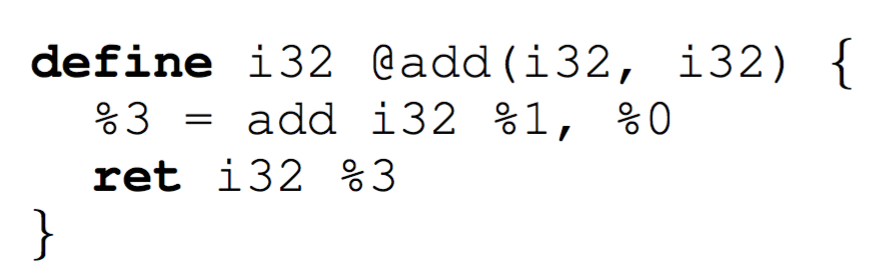
\includegraphics[width=0.4\textwidth]{fig/adaptive-code1.png}
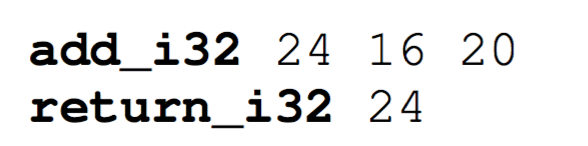
\includegraphics[width=0.28\textwidth]{fig/adaptive-code2.png}
\end{figure} 
\pause
\large{Conventional design!}
\end{frame}

\begin{frame}{Optimization}
Linear-Time Liveness Computation
\begin{itemize}
\item Traditional method has O($n^2$) which is not tolerable
\item New method needs basic blocks in reversed postorder and dominator trees
\end{itemize}
\pause
\hgr{Questions}
\begin{itemize}
\item An iteration-based fix-point solver may be faster
\item Computing dominator trees directly requires O($n^2$)
\end{itemize}
\end{frame}

\begin{frame}{Evaluation}
Show TPC-H results
\begin{figure}[htb]
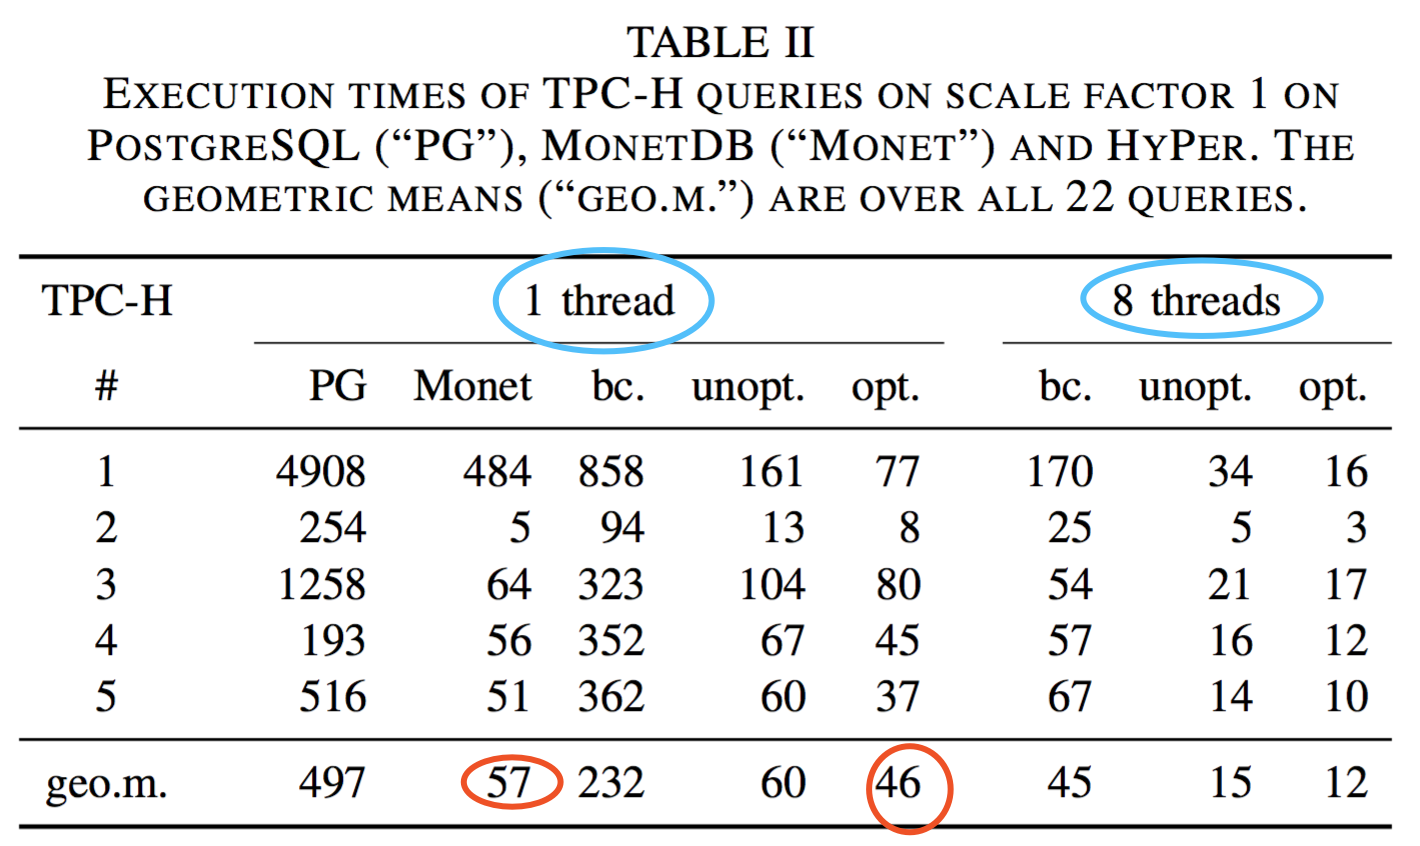
\includegraphics[width=0.6\textwidth]{fig/adaptive-table2.png}
\end{figure} 
\begin{itemize}
\item In 1 thread, opt. is 19\% faster than MonetDB
\item The performance of byte code has been improved a lot with 8 threads.
\end{itemize}
\end{frame}

\begin{frame}{Summary}
Brief summary
\begin{itemize}
\item Interpretation and compilation are both important
\item Adaptive execution with three modes
\item Flexible capability of processing data ranging from 10MB to 30GB
\end{itemize}
\pause
What we learn
\begin{itemize}
\item Switching between different modes may benefit the performance of overall system
\item HorseIR naturally has \texttt{morsels} which are primitive functions
\end{itemize}
\end{frame}
